%!TEX root = ../paper.tex

\section{Evaluation}
\label{sec:evaluation}

The following sections show the evaluation of our approach.
We start with defining relevant evaluation measures and then evaluate our two classifiers and relevant design decisions.

\subsection{Evaluation measures}
\label{sub:evaluation_measures}
We will use the following measures to evaluate our approach:
As already mentioned in a previous section, the demand classifier can be optimized for either precision or recall, depending on the use case.
Therefore, we consider three values:
\begin{itemize}
	\item
		\emph{Precision of demand posts}
		$P_{demand} = \frac{correct~predicted~demands}{predicted~demands}$
	\item
		\emph{Recall of demand posts}
		$R_{demand} = \frac{correct~predicted~demands}{all~demand~posts}$
	\item
		\emph{Overall precision}
		$P_{all} = \frac{correct~predictions}{all~predictions}$
\end{itemize}
This measures capture the most important aspects of our system: If we predict a demand, how likely is it really a demand post, and how many of all demand posts can we actually find.
Finally, the overall precision is usually quite high because of the data skew in the demand tagging.
A tagger, which always returns ``no-demand'' will have an overall precision of \todo{percent}, as seen in Table~\todo{NUMBER}.
However, we left this in for the sake of completeness.

Since there is no such data skew in the product classifier, we just consider the overall accuracy, i.e. what percentage of our predictions were correct.

\begin{figure}
	\label{fig:product_eval}
	\begin{center}
		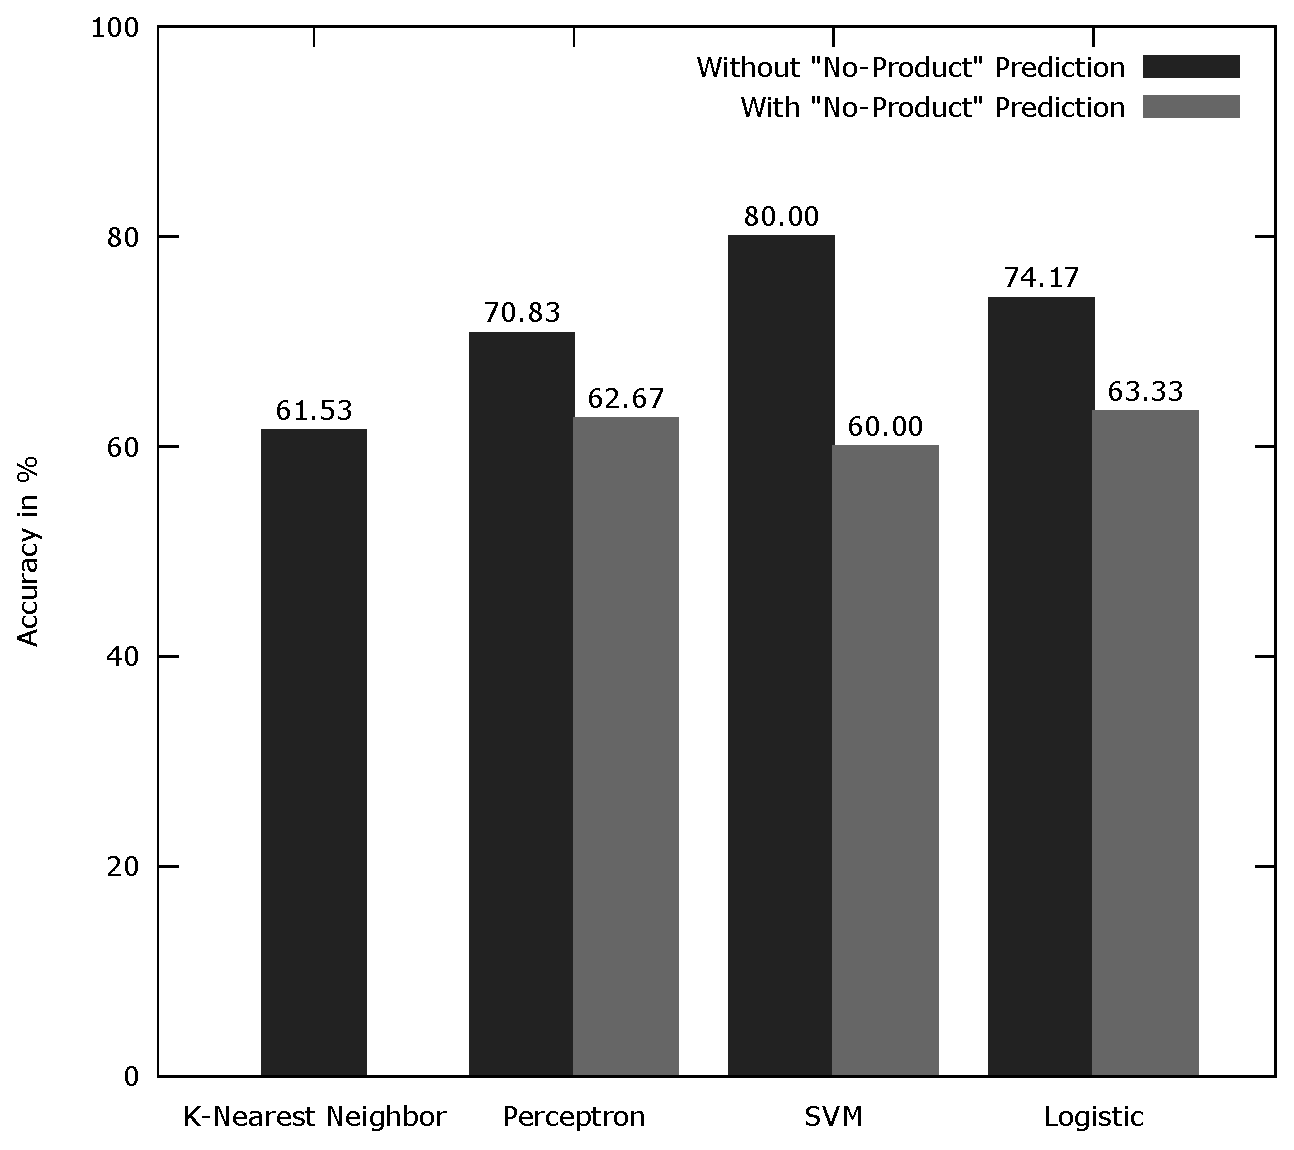
\includegraphics[width=0.7\textwidth]{figures/product_eval.eps}
	\end{center}
	\caption{TODO}
\end{figure}

\begin{figure}
	\label{fig:product_translate_amazon_with_none}
	\begin{center}
		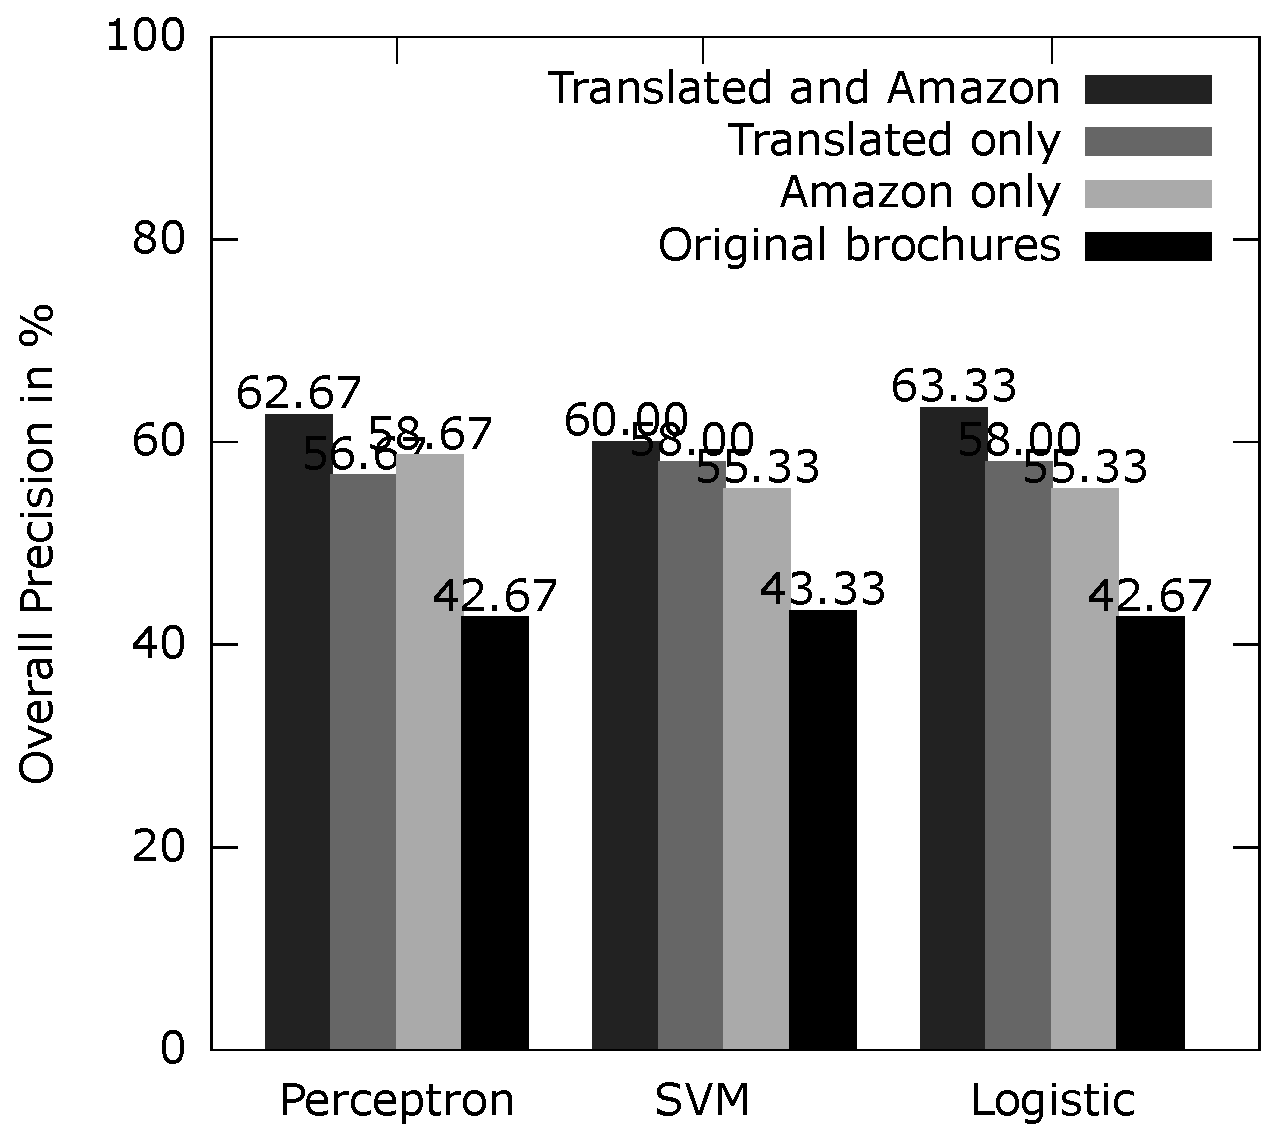
\includegraphics[width=0.7\textwidth]{figures/product_translate_amazon_with_none.eps}
	\end{center}
	\caption{TODO}
\end{figure}

\begin{figure}
	\label{fig:product_translate_amazon_without_none}
	\begin{center}
		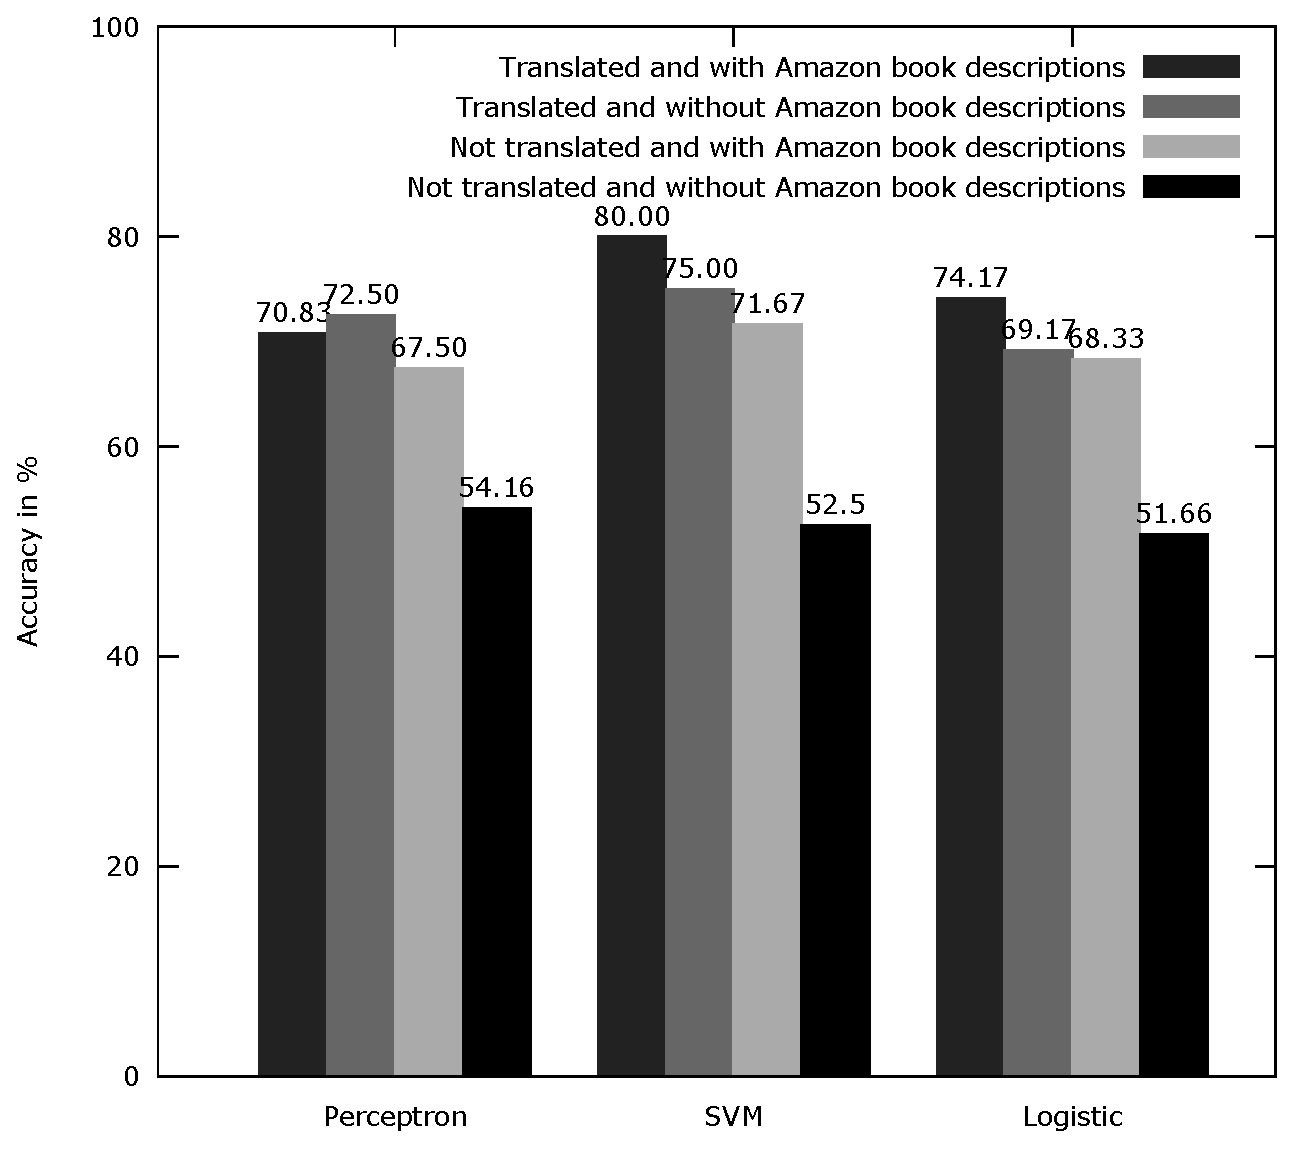
\includegraphics[width=0.7\textwidth]{figures/product_translate_amazon_without_none.eps}
	\end{center}
	\caption{TODO}
\end{figure}

\begin{figure}
	\label{fig:product_feature_selection_with_none}
	\begin{center}
		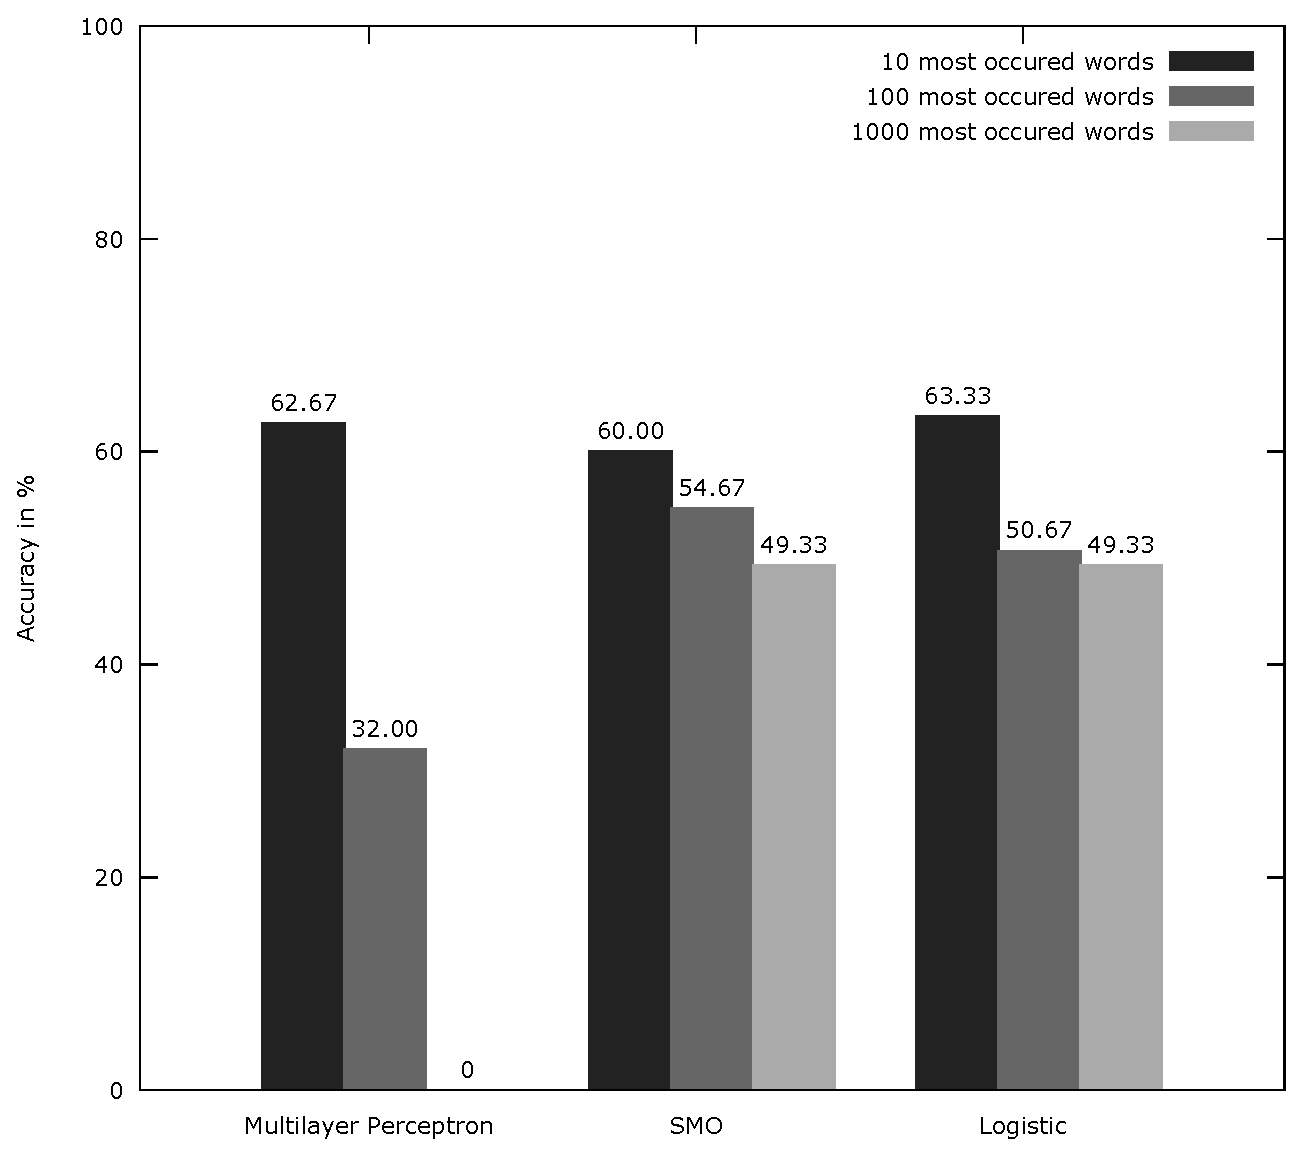
\includegraphics[width=0.7\textwidth]{figures/product_feature_selection_with_none.eps}
	\end{center}
	\caption{TODO}
\end{figure}

\begin{figure}
	\label{fig:product_feature_selection_without_none}
	\begin{center}
		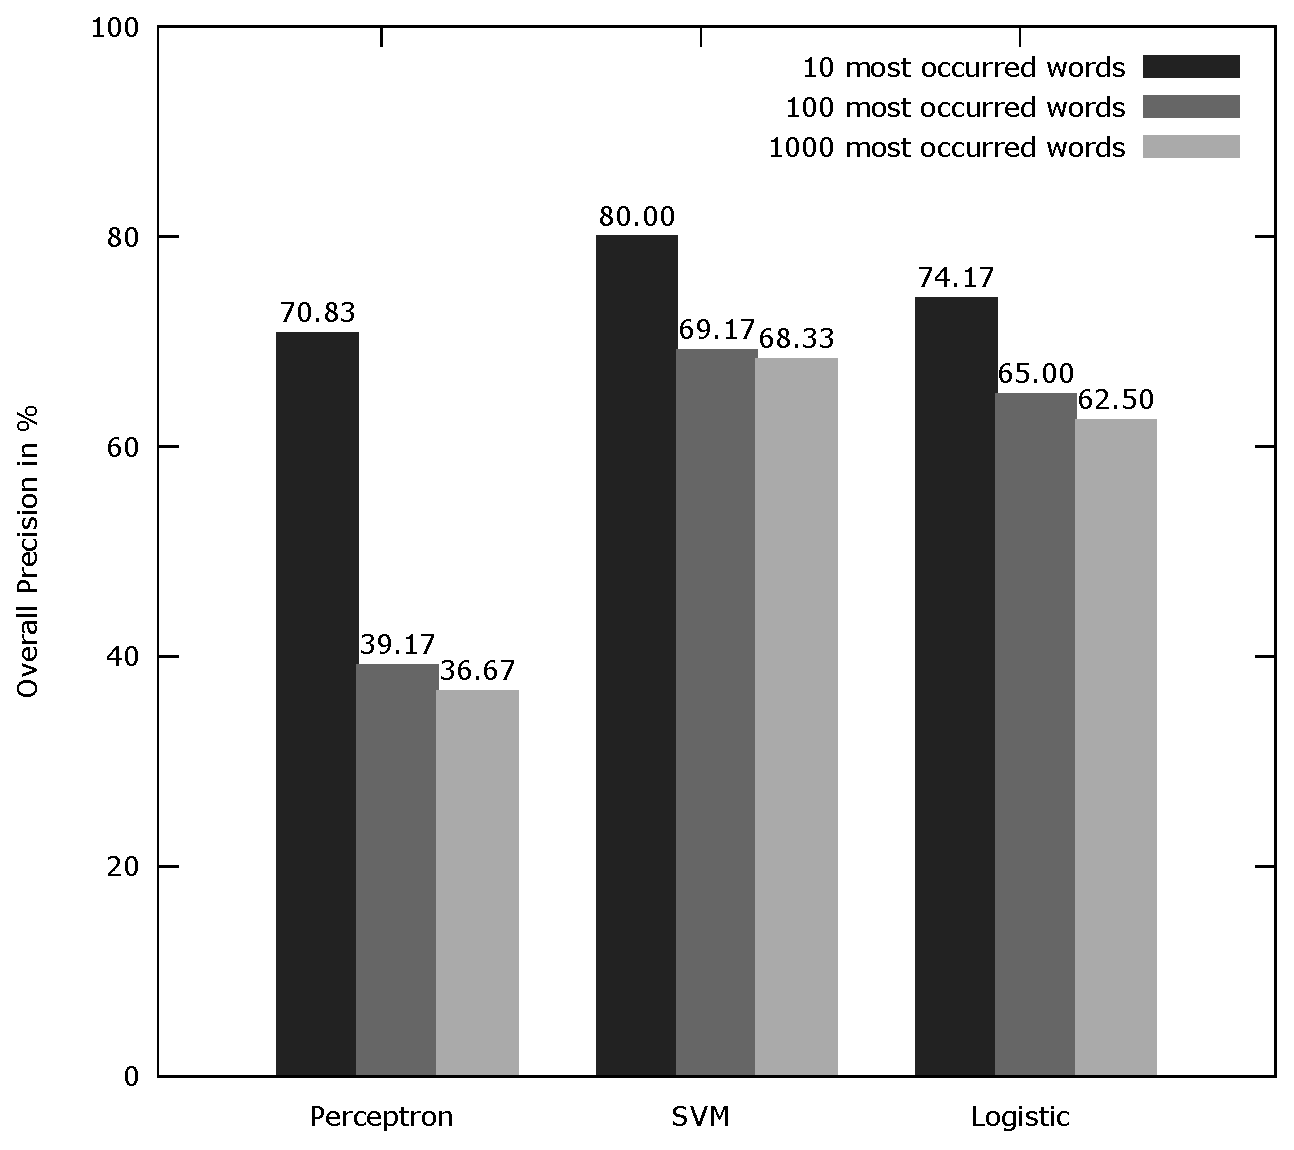
\includegraphics[width=0.7\textwidth]{figures/product_feature_selection_without_none.eps}
	\end{center}
	\caption{TODO}
\end{figure}

\begin{figure}
	\label{fig:sampling_optimization}
	\begin{center}
		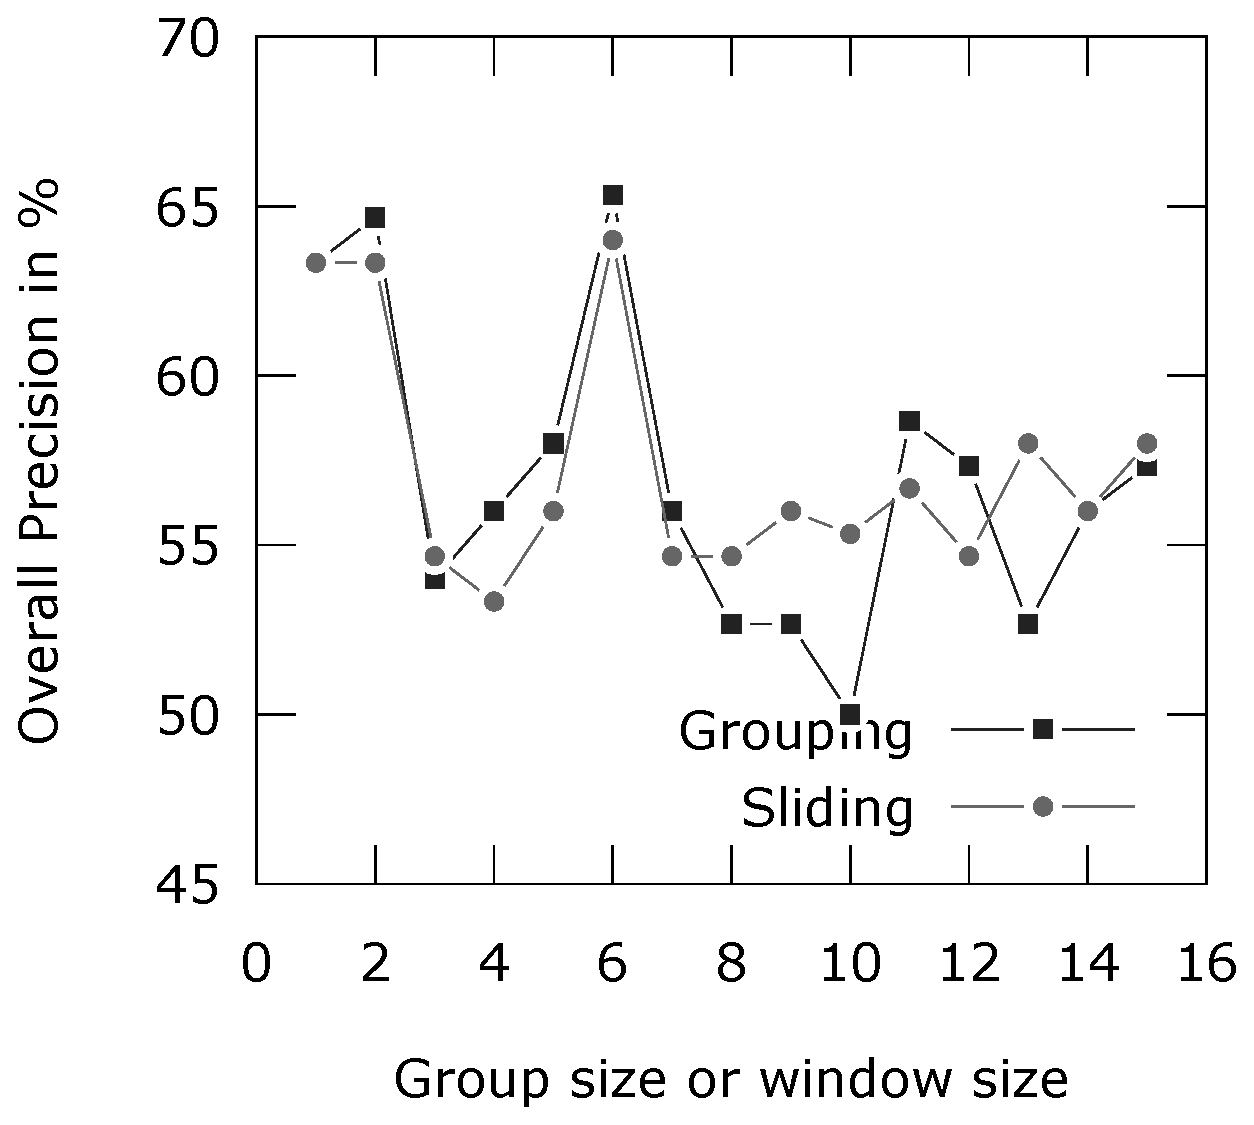
\includegraphics[width=0.7\textwidth]{figures/sampling_optimization.eps}
	\end{center}
	\caption{TODO}
\end{figure}


\subsection{Results}
\label{sub:results}

\subsubsection{Demand classifier}
\label{ssub:demand_classifier}


\subsubsection{Product classifier}
\label{ssub:product_classifier}

\todo{As we said before, linear classifiers performed best for the product classification. As they only have a small difference, we will evaluate on three linear classifiers: logistic regression, perceptron, and support vector machines.}
\subsubsection{Design decision 1: feature selection}

\subsubsection{Design decision 2: splitting size}

\subsubsection{Design decision 3: translation and book descriptions}

Compared with a naive approach, using the brochures as they are, the translation of the German brochures and the enlargement of the training brings an improvement of ...\% for the demand classifier as it is shown in the table \ref{table:demand_trainset_enlargement}.

\endinput
\begin{itemize}
	\item Introduce our data set (show numbers, show examples)
	\item How we got our training data (everything at least twice, use the demands for learning, use the products for evaluation, Active Learning approach)
	\item Reference Precision/Recall from above again, final
	\item Evaluate of the training data generation, which approach is best (random, grouping)
\end{itemize}


